
\chapter{Grundlagen}
\begin{itemize}
	\item im nachfolgenden Erklärungen zu den grundlegenden Konzepten der Arbeit
\end{itemize}
\section{Kompression von Daten}
\subsection{VByte}
\subsection{Lauflängenkodierung}
\begin{itemize}
	\item VByte Kompression
	\item Lauflängenkodierung zur Aggregation von Integern
\end{itemize}
\section{Sicherheit in Datenbanksystemen}
\begin{itemize}
	\item Trusted Computing Base (TCB)
\end{itemize}
\section{Intel Software Guard Extensions}
\begin{itemize}
	\item erstmals 2013 beschrieben
	\item offiziell unterstützt seit der 6. Generation von Intel Core Prozessoren (Codename Skylake), herausgekommen 2015
\end{itemize}
\section{Verwandte Arbeiten}
\begin{itemize}
	\item bei Lösung des Problems der sicheren Datenhaltung und -verarbeitung lassen sich vergangene Ansätze grundsätzlich in zwei Kategorien unterteilen
	\item beide setzen auf eine Verschlüsselung und Auslagerung der Datenbank, sprich Datenverarbeitung findet in gesonderter Komponente statt
	\item 1. Kategorie: direktes Arbeiten auf verschlüsselten Daten unter Nutzung von gewissen Verschlüsselungsschemata die jene Operationen erlauben
	\item 2. Kategorie: Daten werden in gewisse vertrauliche Bereiche transferiert, d.h. dort entschlüsselt, verarbeitet und vor dem Verlassen wieder verschlüsselt
	
	% TODO Usage of subsubsections? Additional level of content?
	%\subsubsection{CryptDB}
	
	\item bekannter Vertreter der 1. Kategorie -> CryptDB
	\item Architektur von CryptDB sieht vor, dass ein vertrauenswürdiger Proxy zwischen der verschlüsselten Datenbank (Datenbankserver) und dem Client steht
	\item Proxy übersetzt: (a) Datenbankanfragen des Clients in eine verschlüsselte Form (b) Ergebnisse der Datenbank in Klartextform %TODO Nachschauen: im Proxy oder erst in Client?
	\item Besonderheit: Nutzung eines speziellen Verschlüsselungsschemas, welches die Auswertung von Anfragen auf verschlüsselten Daten erlaubt
	\item Daten müssen demnach während der Verarbeitung nicht komplett entschlüsselt werden
	\item %TODO Onion scheme
\end{itemize}

\begin{figure}[h]
	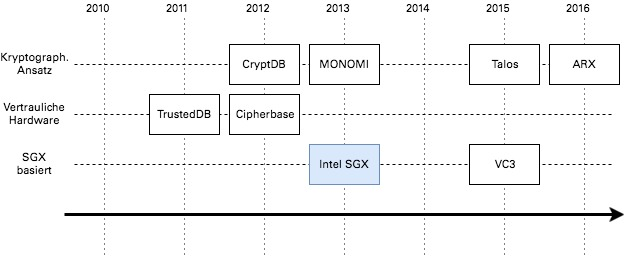
\includegraphics[width=0.9\linewidth]{img/RelatedWorkTimeline.pdf}
	\centering
	\caption{Zeitliche Einordnung nach Kategorie}
	\label{fig:timeline}
\end{figure}
